\subsection{Vue d'ensemble}
Dans les profondeurs de la Terre, du pétrole et du gaz naturel se retrouvent piégés.
%
Ces sources d'énergies sont le résultat de la transformation de matière organique, provenant de végétaux et d'animaux morts, sous très fortes contraintes durant des millions d'années.
%
Bien caché sous des kilomètres de roches, des compagnies pétrolières, comme Total SA, essayent de toutes les trouver avant une compagnie concurrente.


Plus généralement, nous appelons réservoir d'hydrocarbure, ou simplement réservoir, une concentration majeure de pétrole et/ou de gaz naturel sous le sol.
%
La première étape pour trouver un réservoir consiste à analyser le sous-sol avec des ondes acoustiques.
%
Ces ondes sont générées par des explosions pour les analyses sous la mer ou avec un camion sismique pour la surface de la Terre.
%
Ces ondes sont ensuite analysées avec des logiciels de modélisation basés sur les équations des ondes, les compagnies pétrolières peuvent ainsi obtenir une bonne représentation du sous-sol.
%
Après analyse de cette représentation, des puits d'explorations sont forés pour s'assurer de la présence de pétrole.
%
Quand un réservoir est trouvé, l'une des premières questions est : ``Est-il rentable d'exploiter ce réservoir ?''.
%
La simulation de réservoir est un des outils permettant de répondre à cette question.
%
En faisant une simulation de fluides en milieu poreux, les compagnies pétrolières peuvent obtenir une approximation de la quantité d'huile pouvant être récupérée.
%
Si l'exploitation du réservoir est rentable, les compagnies pétrolières commencent l'exploitation.


Mais il ne suffit pas de creuser et d'attendre que le pétrole jaillisse sous la forme d'un geyser comme nous pouvons le voir dans certains cartoons.
%
Les compagnies pétrolières doivent installer des puits.
%
Les puits peuvent être catégorisés en deux catégories majeures (Fig .\ref{fig:wells}) :
%
\begin{itemize}
  \item les puits injecteurs, ce sont les puits qui augmentent la pression à l'intérieur du réservoir en injectant de la matière (eau, gaz(CO$_2$), polymère, ...);
  \item les puits producteurs, ce sont les puits qui récupèrent l'huile, ils sont aussi essentiels au contrôle de la pression en produisant plus ou moins d'huile et de gaz.
\end{itemize}

%   (-_-)   %
\begin{figure}[!ht]
  \centering
  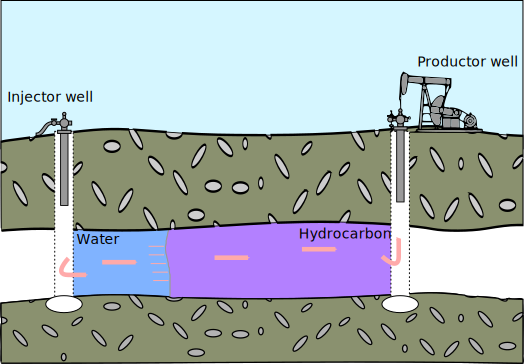
\includegraphics[width=0.8\textwidth]{wells}
  \caption{Exemple d'un champ avec deux puits.}
\label{fig:wells}
\end{figure}


L'une des activités des ingénieurs réservoir consiste à trouver le nombre optimal de puits ainsi que l'emplacement optimal de chacun pour exploiter le réservoir.
%
Encore une fois, la simulation de réservoir leurs permet de tester différentes configurations de placement des puits.
%
Plus tard, quand la compagnie pétrolière a commencé à exploiter le champ, il est intéressent d'avoir des prévisions sur la production d'huile.
%
Une fois de plus, ces résultats sont obtenus avec une simulation de réservoir (Fig. \ref{fig:floviz}).

%   (-_-)   %
\begin{figure}[!ht]
  \centering
  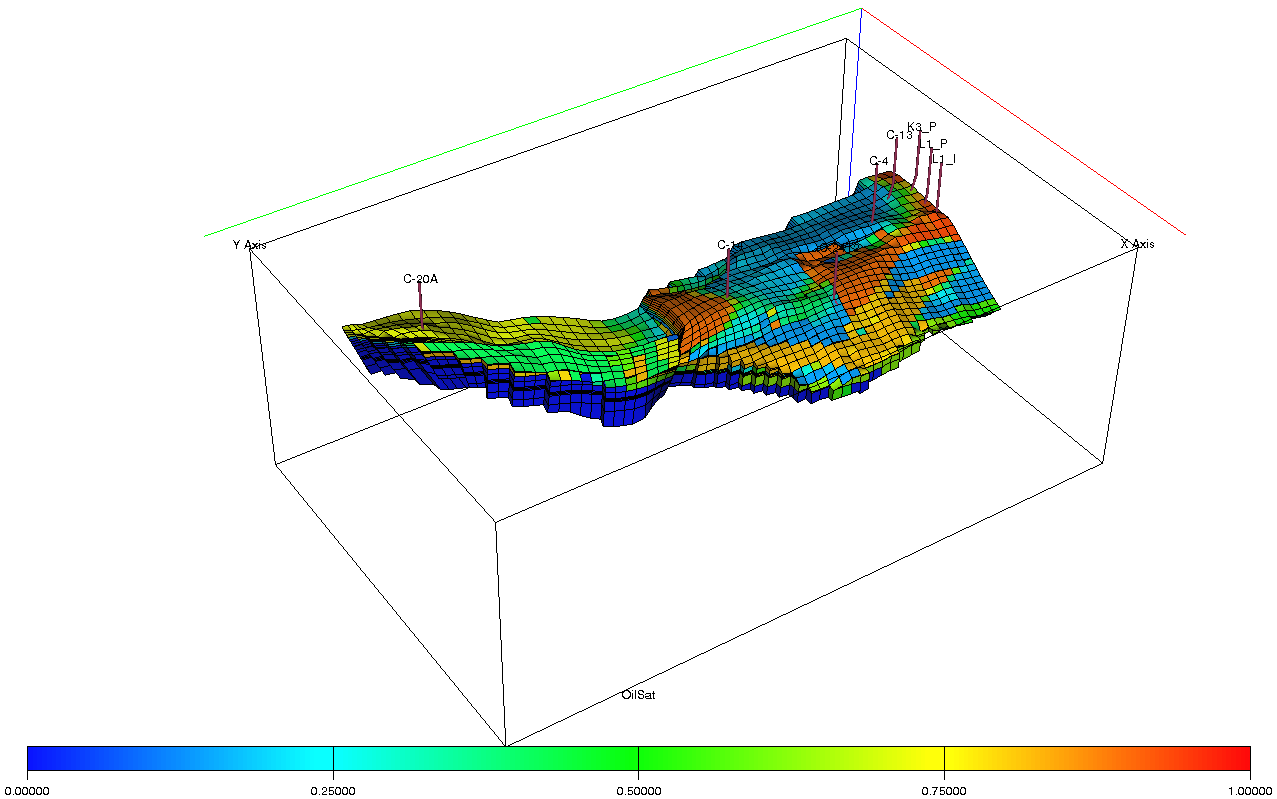
\includegraphics[width=\textwidth]{reservoir}
  \caption{Visualisation de la quantité d'huile dans le réservoir, l'image provient du logiciel floviz.}
\label{fig:floviz}
\end{figure}

Comme montré précédemment, la simulation de réservoir est une étape clé dans le processus de récupération d'hydrocarbures.
%
Il est intéressant pour une compagnie pétrolière de simuler de plus en plus précisément l'intérieur d'un réservoir et bien sûr le simuler aussi vite que possible.
%
Focalisons-nous sur la structure interne d'un simulateur de réservoir.
